\documentclass[tikz,border=3mm]{standalone}
\usetikzlibrary{arrows.meta, positioning}

\begin{document}
    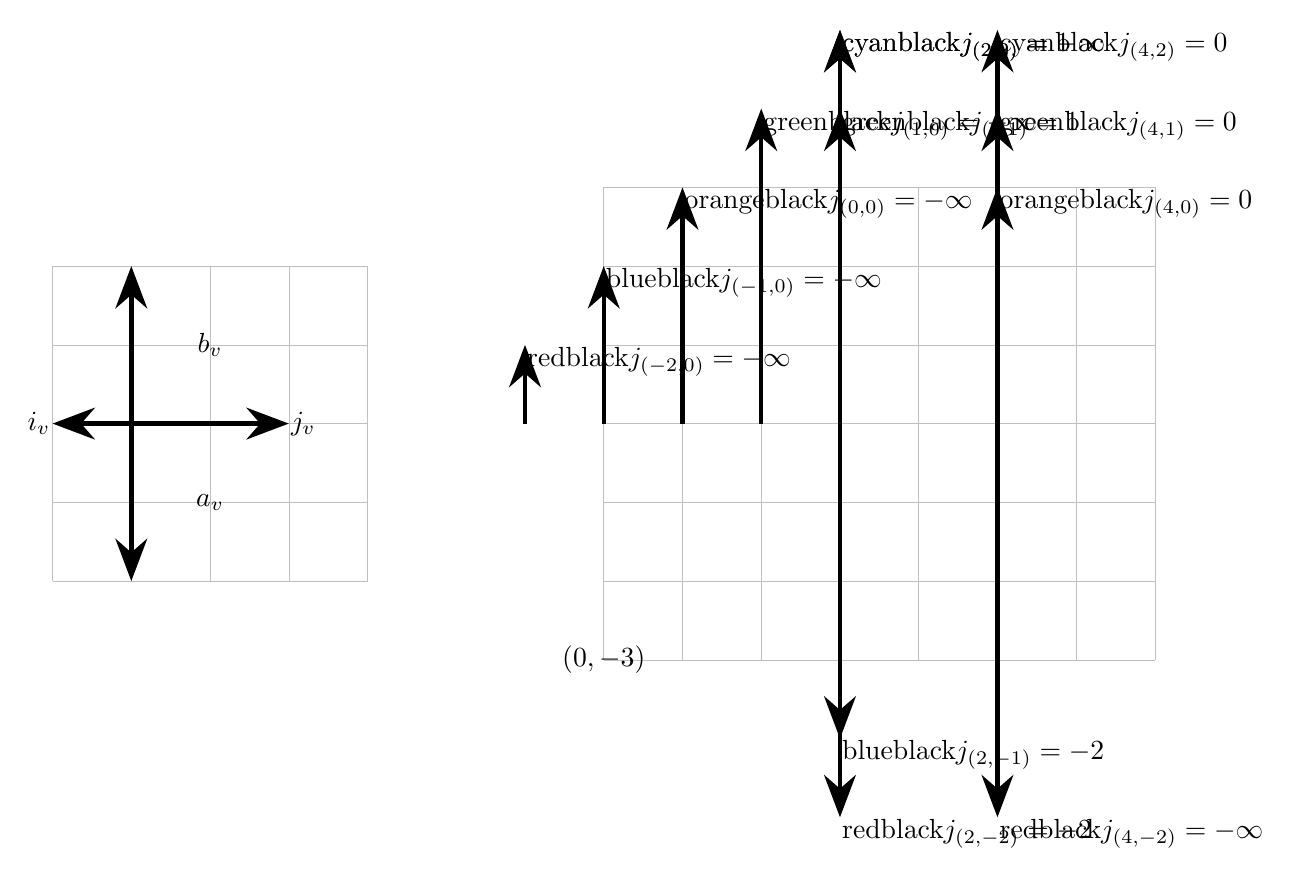
\begin{tikzpicture}[
        >=Stealth,
        every node/.style={inner sep=0pt},
        myline/.style={ultra thick, -{>[scale=1.5]}},
        myarrow/.style={myline, #1},
        mygrid/.style={gray!50, very thin},
    ]

    % Left part: Vertex labels
    \begin{scope}[local bounding box=left]
        \draw [mygrid] (-1,-2) grid (3,2);
        \node (a_v) at (1,-1) {$a_{v}$};
        \node (b_v) at (1, 1) {$b_{v}$};
        
        \draw [myarrow=black] (0,0) -- ++(-1,0) node[left] {$i_{v}$};
        \draw [myarrow=black] (0,0) -- ++(0,-2);
        \draw [myarrow=black] (0,0) -- ++(2,0) node[right] {$j_{v}$};
        \draw [myarrow=black] (0,0) -- ++(0,2);
    \end{scope}

    % Right part: Stochastic six-vertex model
    \begin{scope}[shift={(7cm,0)}, local bounding box=right]
        \draw [mygrid] (-1,-3) grid (6,3);
        \foreach \y/\color in {-2/red, -1/blue, 0/orange, 1/green, 2/cyan}{
            \draw [myarrow=\color] (\y,0) -- ++(0,\y+3) node[below right, black] {$j_{(\y,0)}=-\infty$};
            \ifnum\y>-1
                \draw [myarrow=\color] (4,0) -- ++(0,\y+3) node[below right, black] {$j_{(4,\y)}=0$};
            \fi
            \ifnum\y>0
                \draw [myarrow=\color] (2,0) -- ++(0,\y+3) node[below right, black] {$j_{(2,\y)}=1$};
            \fi
            \ifnum\y<0
                \draw [myarrow=\color] (2,0) -- ++(0,\y-3) node[below right, black] {$j_{(2,\y)}=-2$};
            \fi
            \ifnum\y<-1
                \draw [myarrow=\color] (4,0) -- ++(0,\y-3) node[below right, black] {$j_{(4,\y)}=-\infty$};
            \fi
        }
        
        \node at (-1,-3) {$(0,-3)$};
    \end{scope}
    
    \end{tikzpicture}
\end{document}